\documentclass[UKenglish]{beamer}
\usepackage{pres_preamble}
\usetheme{UiB}


%----------------------------------------------------------------------------------------
%	TITLE PAGE
%----------------------------------------------------------------------------------------

\title{Lorentzian Geometry and Topological Electromagnetism}

\author{Colin Roberts}
\setbeamercolor{title}{fg=white} 
\setbeamercolor{subtitle}{fg=white} 


%----------------------------------------------------------------------------------------
%	PRESENTATION SLIDES
%----------------------------------------------------------------------------------------

\begin{document}

%----------------------------------------------------------------------------------------
%  Thanks and funding
%----------------------------------------------------------------------------------------

\begin{frame}{}
    Thanks and funding
    \begin{figure}[h]
    
\includegraphics[scale=.05]{figures/NASA_logo.svg.png}
    \end{figure}
\end{frame}


%----------------------------------------------------------------------------------------
\section{Introduction}
%----------------------------------------------------------------------------------------



\begin{frame}{Outline}
\vfill
\begin{enumerate}
    \item Intro Lorentzian geometry
    \item de Rham (Co)homology
    \item Topological electromagnetism
    \item Poincar\'e group $\A(1,3)$ and its Lie algebra $\alg(1,3)$
\end{enumerate}
\vfill
\end{frame}


%----------------------------------------------------------------------------------------
\section{Lorentzian Geometry}
%----------------------------------------------------------------------------------------
%
%\begin{frame}{Lorentzian Geometry}
%    
%\end{frame}

%----------------------------------------------------------------------------------------
\section{de Rham (Co)homology}
%----------------------------------------------------------------------------------------


%----------------------------------------------------------------------------------------
\section{Poincar\'e Group}
%----------------------------------------------------------------------------------------

\begin{frame}{}
symmetries of lorentz space.
\end{frame}

%%%%%%%%%%%%%%%%%%%%%%%%%%%%%%%%%%%%%%%%%%%%%%%%%%
%%%%%%%%%%%%%%%%%%%%%%%%%%%%%%%%%%%%%%%%%%%%%%%%%%
%
%
%\begin{frame}{Some Pictures}
%    
%    \begin{columns}[c] % The "c" option specifies centered vertical alignment while the "t" option is used for top vertical alignment
%
%    \column{.25\textwidth}
%    
%    \begin{center} \textbf{Gauss's Laws}
%    
%    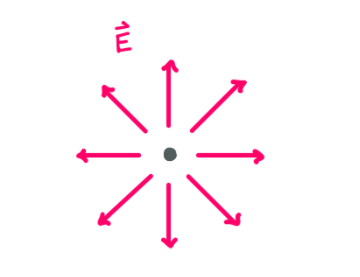
\includegraphics[scale=.4]{figures/gauss i.png}
%    
%    \vspace{-10mm}
%    
%    \small
%    $$ \vec{\nabla} \cdot \vec{E} = \rho(\vec{x},t) $$
%    
%    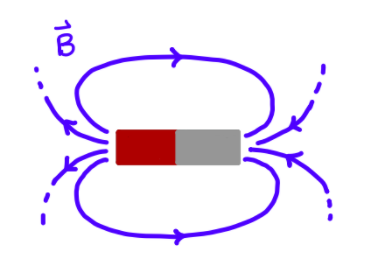
\includegraphics[scale=.4]{figures/gauss ii.png}
%    
%    \vspace{-10mm}
%    
%    $$ \vec{\nabla} \cdot \vec{B} = 0 $$
%    
%    \end{center}
%    
%    \column{.3\textwidth}
%    
%    \begin{center}
%    
%    \textbf{Ampere's Law}
%    
%    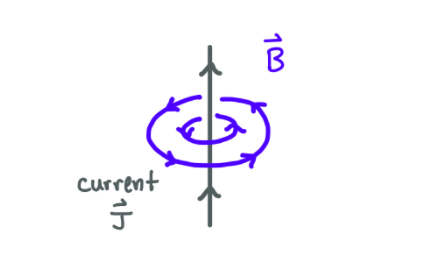
\includegraphics[scale=.4]{figures/ampere.png}
%    
%    \vspace{-10mm}
%    
%    \small
%    $$ \vec{\nabla} \times \vec{B} - \frac{\partial \vec{E}}{\partial t} = \vec{J}(\vec{x},t) $$
%    
%    \normalsize
%    
%    \textbf{Faraday's Law}
%    
%    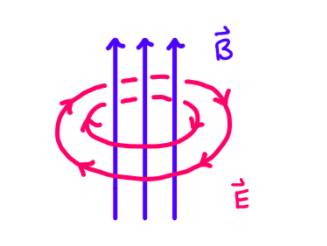
\includegraphics[scale=.4]{figures/faraday.png}
%    
%    \vspace{-10mm}
%    
%    \small
%    $$ \vec{\nabla} \times \vec{E} + \frac{\partial \vec{B}}{\partial t} = 0 $$ 
%    \normalsize
%    
%    \end{center}
%    
%    \column{.45\textwidth}
%    
%    \begin{center}
%        
%        \textbf{Boltzmann / Kinetic Equation}
%        
%        
%        \small
%    $$ \frac{\partial f}{\partial t} + \vec{v} \cdot \frac{\partial f}{\partial \vec{x}} + \frac{e}{m} \left(\vec{E} + \vec{v}\times \vec{B}\right) \cdot \frac{\partial f}{\partial \vec{v}} = 0 $$
%        
%    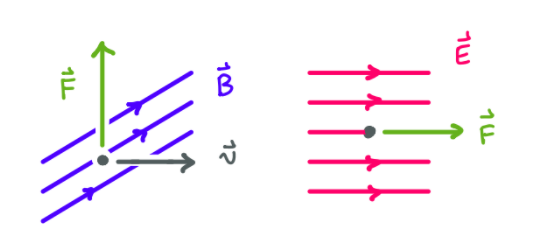
\includegraphics[scale=.5]{figures/lorentz force.png}
%        
%    \end{center}
%    
%    \end{columns}
%    
%    
%\end{frame}
%
%\section{(Co)homology}
%%%%%%%%%%%%%%%%%%%%%%%%%%%%%%%%%%%%%%%%%%%%%%%%%%
%% singular (co)homology
%%%%%%%%%%%%%%%%%%%%%%%%%%%%%%%%%%%%%%%%%%%%%%%%%%
%
%\begin{frame}{Recall: Singular (Co)homology}
%    
%Let $M^n$ be a manifold and let $R$ be a ring.
%
%\textbf{Singular Homology:}
%
%\begin{itemize}
%    \item $C_k(M^n)$: free $R$ module of $k$-chains
%    \item $R$-linear boundary map $\partial_k\colon C_k(M^n)\to C_{k-1}(M^n)$
%\end{itemize}
%
%Then define
%\begin{itemize}
%    \item $\image(\partial_{k+1})$: space of $k$-boundaries
%    \item $\ker(\partial_k)$: space of $k$-cycles
%\end{itemize}
%% Let $R$ be a ring. We can define on $M^n$ the  $C_k(M^n)$ along with the ($R$-linear) boundary operator $\partial_k\colon C_k(M^n)\to C_{k-1}(M^n)$.
%% Define the space of $k$-boundaries to be $\image(\partial_{k+1})$ and the space of $k$-cycles to be $\ker(\partial_k)$.
%Since $\partial^2 = 0$, we can form a chain complex and take its singular homology, with
%\begin{equation*}
%    \label{eq:singular_homology}
%    H_k(M^n;R) \coloneqq \bigslant{\ker(\partial_{k})}{\image(\partial_{k+1})}.
%\end{equation*}
%
%\textbf{Singular Cohomology:}
%
%\begin{itemize}
%    \item $C^{k}(M^n)\coloneqq \hom(C_k(M^n),R)$: space of cochains
%    \item coboundary operator $\partial^k \colon C^{k}(M^n)\to C^{k+1}(M^n)$
%\end{itemize}
%
%% Dually, we can form the singular cohomology groups by defining the space of cochains . This gives rise to the coboundary operator . The singular cohomology groups are given by
%\begin{equation*}
%    \label{eq:singular_cohomology}
%    H^k(M^n;R) \coloneqq \bigslant{\ker(\partial^{k})}{\image(\partial^{k-1})}.
%\end{equation*}
%    
%\end{frame}
%
%
%%%%%%%%%%%%%%%%%%%%%%%%%%%%%%%%%%%%%%%%%%%%%%%%%%
%% de Rham
%%%%%%%%%%%%%%%%%%%%%%%%%%%%%%%%%%%%%%%%%%%%%%%%%%
%
%
%\begin{frame}{de Rham (Co)homology}
%\vfill
%\begin{itemize}
%    \item Given a manifold $M$, we have the exterior algebra of (compactly supported) forms $\Omega(M)$.
%    \begin{itemize} 
%        \item de Rham cochain complex is built with the exterior derivative $d$.
%        \item de Rham cohomology ring is
%        \[
%            H^\bullet_{dR}(M) = \bigwedge_{k \in \mathbb{N}} H^k_{dR} = \bigwedge_{k \in \mathbb{N}} \ker d_k ~/~ \im d_{k-1}.
%        \]
%    \end{itemize}
%    \item The dual space $\Omega^*(M)$ is the space of currents $T\colon \Omega(M) \to \R$.
%    \begin{itemize}
%        \item de Rham chain complex is built with boundary operator $\partial$
%        \[
%            \partial T[\alpha] = T[d \alpha].
%        \]
%        \item de Rham homology group is
%        \[
%            H_\bullet^{dR} = \bigoplus_{k\in \mathbb{N}} H_k^{dR} \coloneqq \bigoplus_{k\in \mathbb{N}} \ker \partial_k ~/~ \im \partial_{k+1}. 
%        \]
%    \end{itemize}
%\end{itemize}
%\vfill
%\end{frame}
%
%\begin{frame}{Multivector Equivalents of Forms}
%\vfill
%Given a Riemannian manifold $(M,g)$, take the Clifford algebra bundle $\G(M)$ whose sections are multivector fields.
%\begin{itemize}
%    \item A $k$-form $\alpha_k$ has a multivector equivalent $A_k$ by
%    \[
%    \alpha_k = A_k \cdot dX_k.
%    \] 
%    \begin{itemize}
%        \item $d\alpha_k \mapsto \grad \wedge A_k$.
%        \item $\delta \alpha_k \mapsto \grad \cdot A_k$.
%    \end{itemize}
%    \item de Rham cohomology: $H^\bullet_{dR}(M) \cong \bigoplus_{n\in \mathbb{N}} \ker \grad \wedge_k ~/~ \im \grad \wedge_{k+1}$.
%    \item de Rham homology: $H_\bullet^{dR} = \bigoplus_{k\in \mathbb{N}} \ker \grad\cdot_k ~/~ \im \grad\cdot_{k+1}$. 
%\end{itemize}
%\vfill
%\end{frame}
%
%\begin{frame}{Multivector Equivalents of Currents}
%\vfill
%We have the Riemannian volume form $\mu$ and the bilinear pairing of multivectors $(-,-)$
%\begin{itemize}
%    \item We can take a $k$-current by
%    \[
%    T[-] = \int_M (T_k,-)\mu.
%    \]
%    and for a $k$-chain $K$ we have the $k$-current $\delta_K$
%    \[
%    \delta_K[-] = \int_K \mu_K = \int_M (\blade{I}_K,-)\mu.
%    \]
%    \item The boundary operator acts accordingly
%    \[
%    \partial T[\alpha_{k-1}] = T[d\alpha_{k-1}] = \int_M(T_k,\grad \wedge A_{k-1})\mu = \int_M (\grad \cdot T_k,A_{k-1})\mu
%    \]
%    and by Stokes' theorem
%    \[
%    \partial \delta_K[\alpha_{k-1}]= \int_{\partial K} \alpha_{k-1}.
%    \]
%\end{itemize}
%\vfill
%\end{frame}
%
%\begin{frame}{Useful Theorems}
%\vfill
%
%    \begin{theorem}[de Rham's Theorem]
%        The singular (co)homology over $\R$ is isomorphic to the de Rham (co)homology.
%    \end{theorem}
%    \begin{theorem}[Poincar\'e Duality]
%        We have $H_k\cong H^{n-k}$ by the dual $\perp$. %this is true for forms with compact support
%    \end{theorem}
%    \begin{theorem}
%        The cap product is given by $\rfloor\colon H^\ell(M) \times H_k(M)\to H_{k-\ell}(M)$.
%    \end{theorem}
%
%\vfill
%\end{frame}
%
%%%%%%%%%%%%%%%%%%%%%%%%%%%%%%%%%%%%%%%%%%%%%%%%%%
%\section{Topological Electromagnetism}
%%%%%%%%%%%%%%%%%%%%%%%%%%%%%%%%%%%%%%%%%%%%%%%%%%
%
%
%\begin{frame}{Axioms}
%\vfill
%There are four physical postulates for electromagnetism that we write as topological axioms.    
%    \begin{itemize}
%    \item{\bf{Axiom 1.}} \emph{Conservation of charge:} Current density $\blade{J}_3$ must flow through boundaries of regions $N^4$ so
%    \[
%    0=\int_{\partial N^4} \blade{J}_3\cdot dX_3=\int_{N^4} (\grad \wedge \blade{J}_3) \cdot dX_4
%    \]
%    so $\blade{J}_3$ is closed. Hence, for a co-closed 3-current $\delta_{N^3}$  we have $\delta_{N^3}[j_3]=0$ and which implies the magnetic excitation $H$ is the potential $\grad \wedge H=\blade{J}_3$ or dually $\blade{J}=\blade{J}_3^\perp = \grad \cdot H^\perp$ defines a homology class.
%    \item{\bf{Axiom 2.}} \emph{Conservation of flux:} The electromagnetic field $F$ defines a cohomology class in $H^2(M)$ by taking a co-closed 2-current $N^2$ and noting
%    \[
%    \int_{N^2} F \cdot dX_2 = 0 
%    \]
%    implies $\grad \wedge F=0$.
%\end{itemize}
%\vfill
%\end{frame}
%
%\begin{frame}{Axioms}
%\vfill
%    \begin{itemize}
%    \item{\bf{Axiom 3.}} \emph{Constitutive law:} We relate the excitation $H$ with the field $F$. The simplest case is the linear case given by $F=H^\perp$ which yields the Maxwell equations $\grad F = \blade{J}$ or, in their more recognizable relativistic form
%    \begin{align*}
%        \grad \wedge F &= 0 && \textrm{(homogeneous)}\\
%        \grad \cdot F &= \blade{J} && \textrm{(inhomogeneous)}
%    \end{align*}
%    The homogeneous equations are Gauss's law for magnetism and Faraday's law whereas the inhomogeneous are Gauss's law for electricity and Ampere's law.
%    \item{\bf{Axiom 4.}} \emph{Lorentz force:} The motion of a particle with 4-velocity $\blade{v}$ in a field $F$ is
%    \[
%    \nabla_{\blade{v}}\blade{v} = \frac{q}{m} \blade{v} \cdot F.
%    \]
%\end{itemize}
%\vfill
%\end{frame}
%
%
%\begin{frame}{Mass Hyperboloid}
%\vfill
%\begin{itemize}
%    \item Mass hyperboloid $\Gamma_m\coloneqq \{ \blade{p} \in T_xM^4 ~\vert~ g_x(p,p)=-m^2 \}$
%\end{itemize} 
%\begin{center}
%    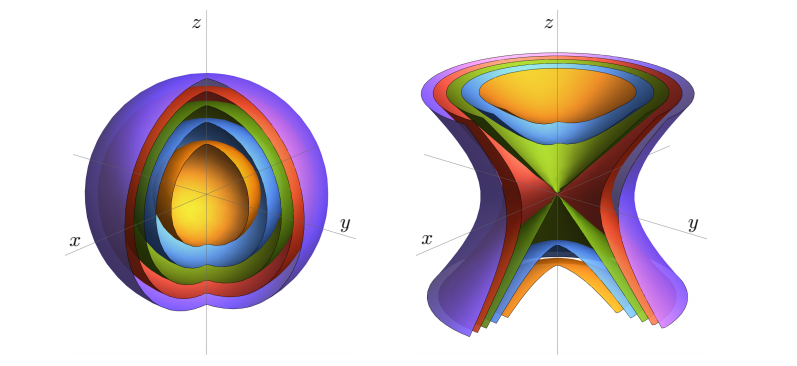
\includegraphics[scale=.5]{presentation/foliations2.png}
%\end{center}
%\vfill   
%\end{frame}
%
%
%\begin{frame}{Mass Hyperboloid Foliation}
%    
%
%    
%\end{frame}
%
%
%
%%%%%%%%%%%%%%%%%%%%%%%%%%%%%%%%%%%%%%%%%%%%%%%%%%
%% Plasma Fluids
%%%%%%%%%%%%%%%%%%%%%%%%%%%%%%%%%%%%%%%%%%%%%%%%%%
%\section{Plasma Fluids}
%
%\begin{frame}{Fermi Transport}
%    \vfill
%    \begin{itemize}
%        \item A particle $\gamma\colon T\to M^4$ of constant mass energy $m$ has a 4-momentum $\dot{\gamma}=\blade{p}=m\blade{v}$
%        \item Mass energy is conserved, $H(x,\blade{p})=\frac{1}{2}g_x(\blade{p},\blade{p})$ is conserved along $\gamma$ hence
%        \[
%            \grad ({\blade{v}} \cdot {\blade{v}}) = 0 ~\implies~ \nabla_{\blade{v}} {\blade{v}} =  {\blade{v}}\cdot \underbrace{(\grad \wedge {\blade{v}})}_{\textrm{vorticity }\omega}
%        \]
%        \item Optimal transport of 4-velocity is given by projection onto the vorticity plane
%        \begin{figure}
%            \centering
%            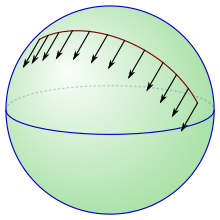
\includegraphics[width=.2\textwidth]{figures/parallel_transport.png}
%        \end{figure}
%        \end{itemize}
%    \vfill
%\end{frame}
%
%\begin{frame}{Classical Fluid Quantities}
%\vfill
%    \begin{itemize}
%        \item Vorticity $\blade{\omega}$ represents rotational fluid motion in a plane
%        \begin{figure}
%    \centering
%    \begin{subfigure}[b]{0.15\textwidth}
%        \centering
%        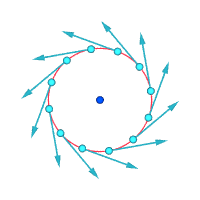
\includegraphics[width=\textwidth]{figures/Vorticity_Figure_01_c.png}
%    \end{subfigure}
%    \hspace*{3cm}
%    \begin{subfigure}[b]{0.15\textwidth}
%        \centering
%        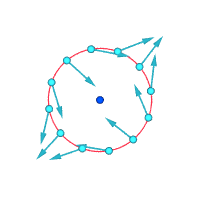
\includegraphics[width=\textwidth]{figures/Vorticity_Figure_02_c.png}
%    \end{subfigure}
%    \end{figure}
%        \item In general, the product of velocity with vorticity decomposes
%        \[
%        \blade{v}\blade{\omega} = \underbrace{\blade{v}\cdot \blade{\omega}}_{\textrm{transport}}+\underbrace{\blade{v}\wedge\blade{\omega}}_{\textrm{helicity}}
%        \]
%            
%        \begin{figure}
%            \centering
%            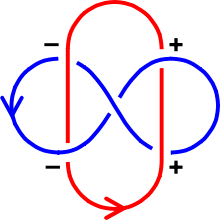
\includegraphics[width=0.15\textwidth]{figures/gauss_linking.png}
%        \end{figure}
%    \end{itemize}
%
%\vfill    
%\end{frame}
%
%%%%%%%%%%%%%%%%%%%%%%%%%%%%%%%%%%%%%%%%%%%%%%%%%%
%
%\begin{frame}{Faraday Transport}
%    \vfill
%    \begin{itemize}
%        \item For a charged particle, we have the Lorentz force law $\nabla_{\blade{v}}\blade{v} = \frac{1}{2} \blade{v}\cdot F$
%        \item In terms of a proper time parameterization $\frac{d\blade{v}}{d\tau} = \frac{1}{2} \blade{v} \cdot F(\gamma(\tau))$.
%    \end{itemize}
%    \begin{figure}
%        \centering
%        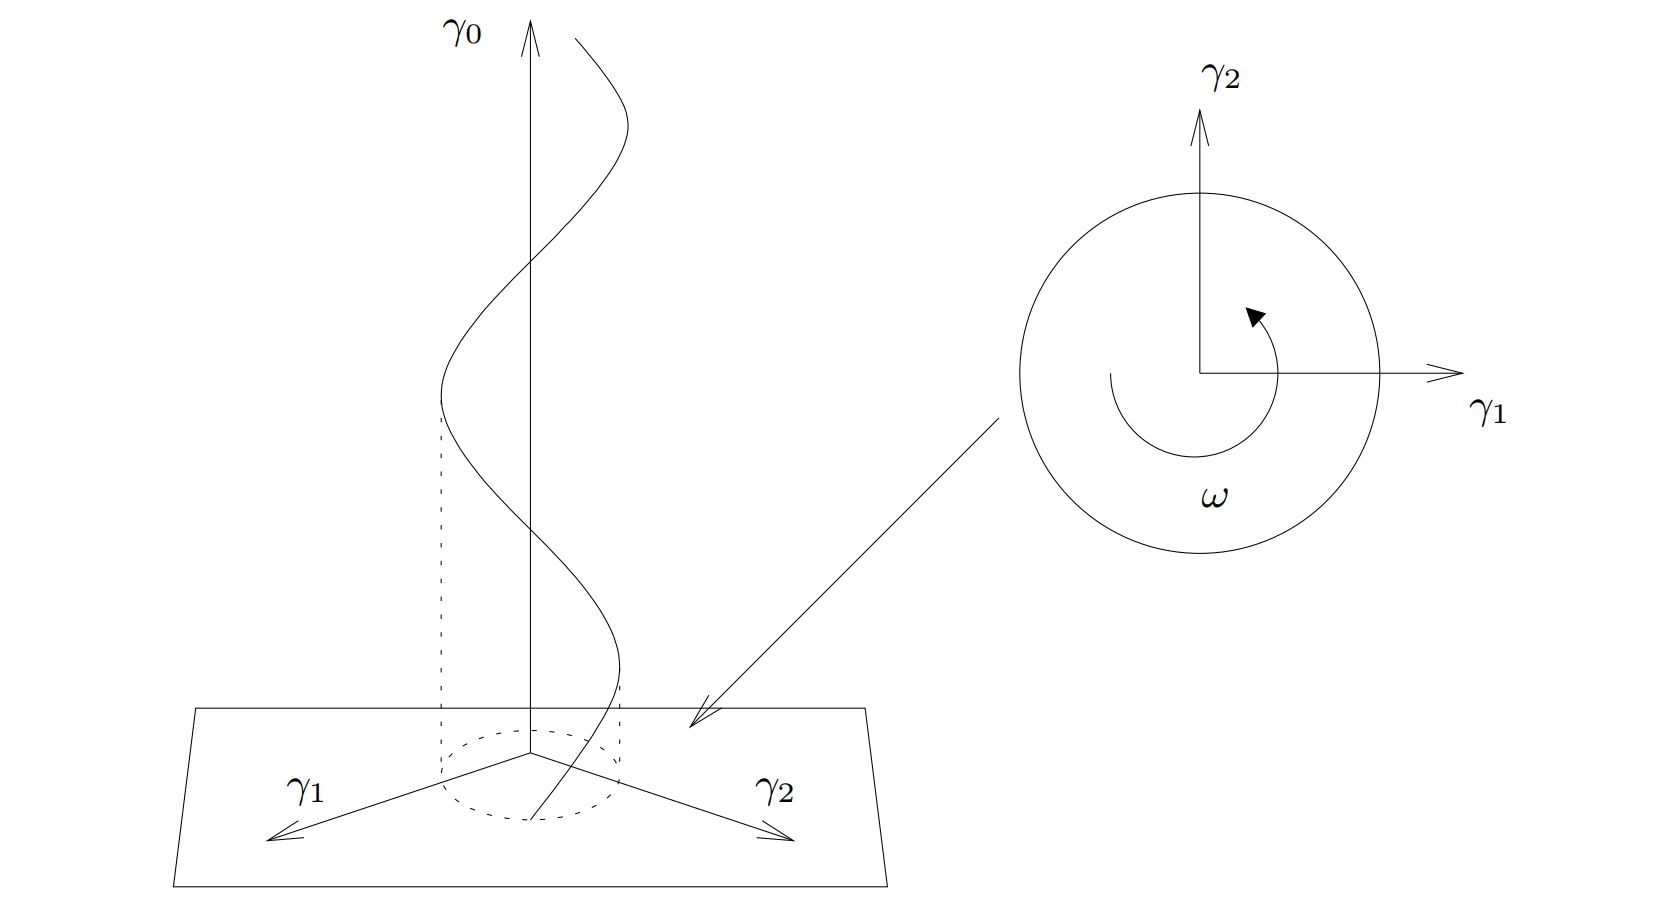
\includegraphics[width=.65\textwidth]{figures/helical_path.png}
%    \end{figure}
%    \vfill
%\end{frame}
%
%\begin{frame}{Spinor Equations}
%    \vfill
%
%    \begin{itemize}
%        \item Since $\blade{v}\cdot\blade{v}$ is constant, velocity at any $\tau$ is given by time varying isometries
%    \[
%    \blade{v}(\tau)=\mathsf{R}_\tau(\blade{v}_0)
%    \]
%    \item Since $R \in \sping(1,3)$ induces $\mathsf{R}(\blade{v}_0)=R\blade{v}_0 R^\dagger$, particle configuration is a curve in the Lie group $\R^{1,3}\rtimes \sping^+(1,3)$ with Lie algebra $\R^{1,3}\rtimes \spina(1,3)$.
%        \begin{figure}
%        \centering
%        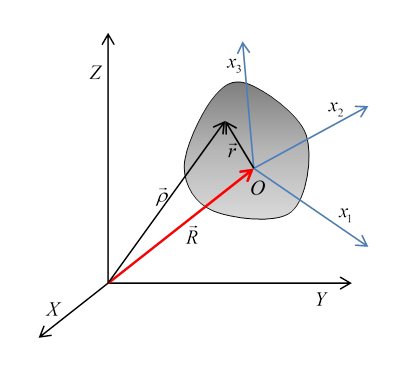
\includegraphics[width=.32\textwidth]{figures/rigid_body.png}
%    \end{figure}
%    \item Fermi-Faraday transport of a spinor is given by $\frac{dR}{d\tau} = FR$
%    \end{itemize}
%    \vfill
%\end{frame}
%
%\begin{frame}{Plasma Fluid}
%    \vfill
%    
%    \begin{itemize}
%        \item Let $m,q\colon N^4 \to \R$ be the mass and charge field and $\blade{v} \in \mathfrak{X}(M)$
%        \item Then the current $\blade{J}=q\blade{v}$
%        \item If we allow mass to flow separately from the velocity 
%        \[
%        \boxed{m\nabla_{\blade{v}}\blade{v} + (\nabla_{\blade{v}}m)\blade{v} = q\blade{v} \cdot \blade{F}}
%        \]
%        \item Assume our axioms of EM so $\grad \cdot \blade{J}=0$ and the constraint that charge to mass is constant yields
%        \[
%        \boxed{\grad \cdot \blade{v} = 0}
%        \]
%        \item Maxwell's equations hold
%        \[
%        \boxed{\grad F = \blade{J}}
%        \]
%    \end{itemize}
%    \vfill
%\end{frame}
%

\end{document}